%%%%%%%%%%%%%%%%%%%%%%%%%%%%%%%%%%%%%%%%%%%%%%%%%%%%%
% Configuration 
%%%%%%%%%%%%%%%%%%%%%%%%%%%%%%%%%%%%%%%%%%%%%%%%%%%%%
 
\documentclass[a4paper, 11pt, french]{article}

\voffset -0cm
\hoffset 0.0cm
\textheight 22cm
\textwidth 16cm
\topmargin 0.0cm
\oddsidemargin 0.0cm
\evensidemargin 0.0cm

\usepackage{epsfig}  
\usepackage{setspace}
\usepackage{fancyheadings}
\usepackage{amsmath}
\usepackage{amssymb}
\usepackage{graphicx}


%%%%%%%%%%%%%%%%%%%%%%%%%%%%
%%%%%%% TITRE  %%%%%%%%%%%%%
%%%%%%%%%%%%%%%%%%%%%%%%%%%%

\title{\bf{TD4: Morphological operators, connected components extraction, and persistant homology}}
\author{}
\date{}

%%%%%%%%%%%%%%%%%%%%%%%%%%%
%%% Debut du document %%%%%
%%%%%%%%%%%%%%%%%%%%%%%%%%%


\begin{document}

\maketitle

\begin{figure}[ht]
	\begin{center}
	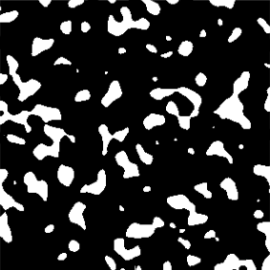
\includegraphics[width=5cm]{cells.png}
	\caption{Test image for granulometry applications. The goal is to see the evolution of the number of cells as the structuring element size grows.}
	\end{center}
\end{figure} 

\par In this TP, we focus will develops the tools needed for persistent homology computations. The ingredients needed are:
\begin{itemize}
\item \textbf{Morphological operators:} The goal is to compute openings as a erosion followed by a dilation. We will focus on binary images.
 \item \textbf{A connected component counter:} The goal is be able to determine the number of connected components in a binary image.
 \item \textbf{Persistent homology:} The goal is to see the evolution of the number of connected components as the structuring element size increases.
\end{itemize}

\section*{Morphological operators}

The first tool you will need to implement is the opening morphological operator. This requires implementing the erosion and dilation operators. We recall that, given a binary structuring element $S$ of size $k \times k$ and a grayscale image $I$, the erosion operator produces an image $E$ such that $E(x,y) = \min_{\{m,n | S(m,n)=1\}} \{I(x+m, y+n)\}$ and the dilation operator $D$ is $D(x,y) = \max_{\{m,n | S(m,n)=1\}} \{I(x+m, y+n)\}$.

Implement the opening operator, which consists in an erosion followed by a dilation.

For a preliminary implementation of persistent homology, plot the curve : $\#white pixels = f(k)$. 



% =======================================================================
\section*{Exercise 2 \rm Connected components by double-scan}


\par The algorithm consists on a two-pass scan of the image. During the first scan, we identify potential connected components and during the second one, we validate such components using a relabelling step. The main idea is to scan the image starting from top left using half-connectivity masks (cf Figure \ref{fig:masks}).

\begin{figure}
	\begin{center}
	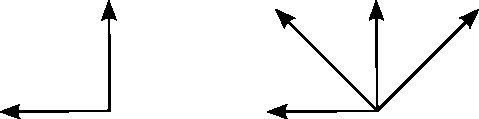
\includegraphics[width=6cm]{masks}
	\caption{Half-mask for the (1)- and (0)-adjacency.\label{fig:masks}}
	\end{center}
\end{figure}

\smallskip
\par In the following, the result of the algorithm will be an image $L$ with one label per connected regions. These labels will be represented by letters. The algorithm is the following
	\begin{itemize}
	\item \textbf{First scan:} We apply one of the two half-masks. For each point $p$:
		\begin{itemize}
		\item If one of its neighbours $q$ has the same gray level, then we propagate the label ($L(p) = L(q)$).
		\item If no neighbour has the same gray level, we create a new label and store it in $L(p)$.
		\item If $p$ has several neighbours with the same gray level but with different labels (labels $a$, $b$), we pick one of them for $p$ (the "lowest" one, for example) and we keep track that both labels correspond to the same region (i.e. $b$ is a synonym of $a$) by a so called \emph{Collision list}. For example, you could propagate the lowest label in the neighbourhood and make all labels in this neighbourhood "point" to the lowest one.
		\end{itemize}
	\item Figure \ref{fig:connected} illustrates the overall process with four temporary labels and only two remain after the pruning step. As illustrated in this figure, you could implement the collision list as a list where each node has a pointer to its \emph{lowest} parent during the first scan.
	
	\item \textbf{Second scan:} Process the collision list such that each label now points to either to itself or to its root (for example, $D$ is now connected to $A$ instead of $C$). Then, for each pixel we simply remap the labels according to the pruned collision list.
	\end{itemize}

\begin{figure}[ht]
	\begin{center}
	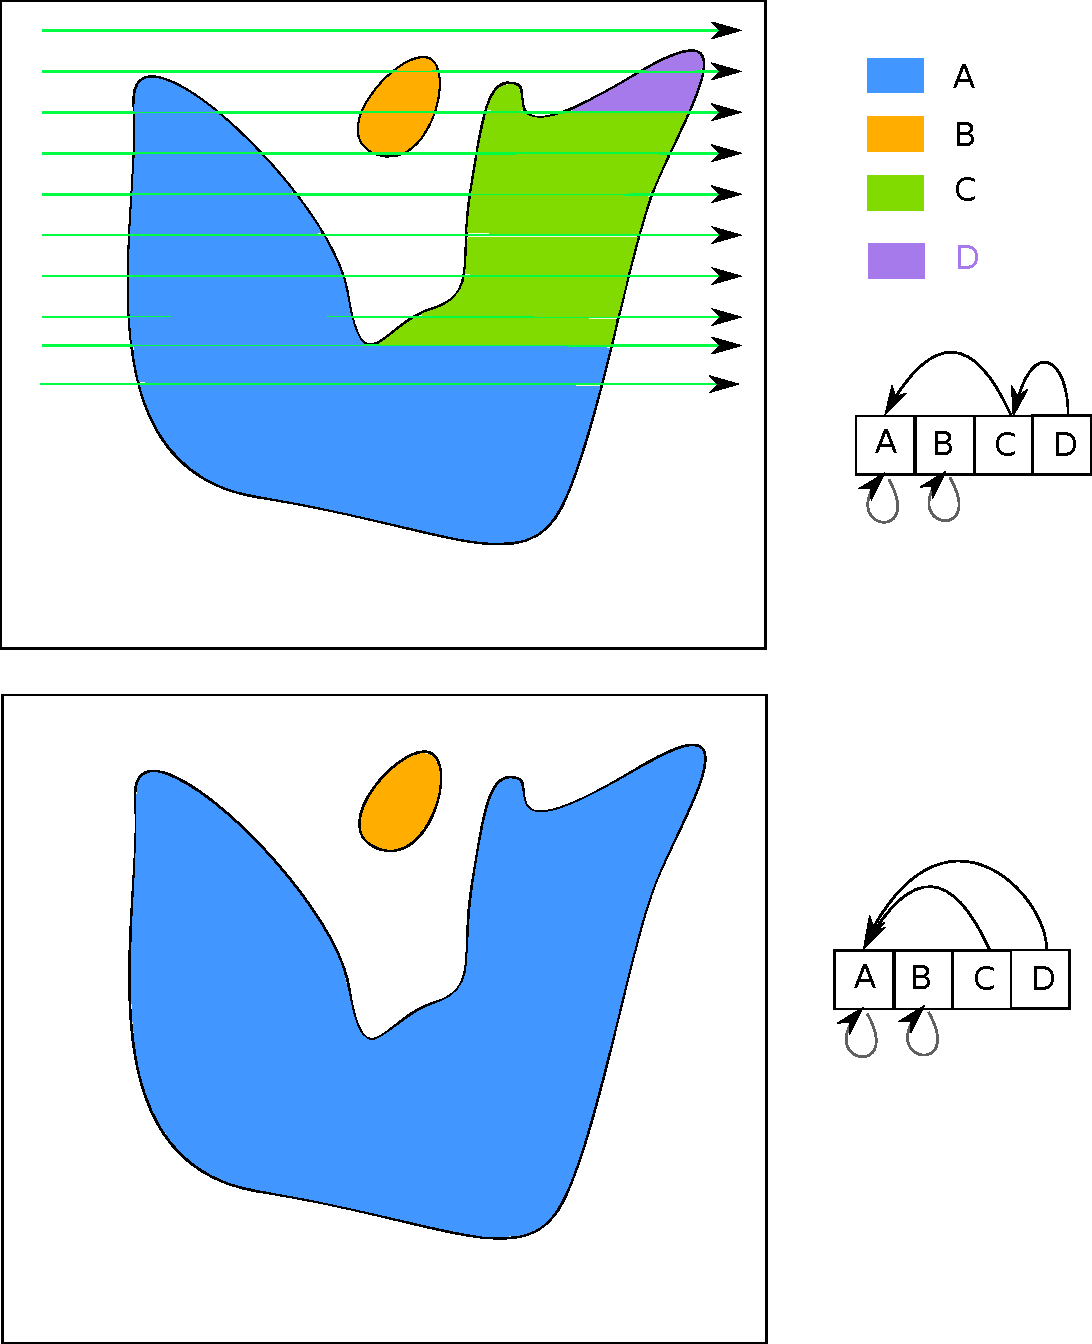
\includegraphics[width=10cm]{connected}
	\caption{Result of the first pass and relabelling.\label{fig:connected}}
	\end{center}
\end{figure}


{\bf Questions:}
\begin{enumerate}
	\item Implement the algorithm described above, for the the $(0)-$ and the $(1)-$adjacencies. Use this algorithm on the provided input png file, then output the label map in png format. 
	\item Ouput the number of connected components
\end{enumerate}



\section*{Exercise 3 \rm Persistent homology}

We are now ready to compute persistent homology and see how the number of connected components of our image varies when increasing the morphological structuring element size.
Progressively increase the size of the structuring element and plot the number of connected components as a function of the structuring element size.	

\end{document}


